\documentclass[conference]{IEEEtran}
\usepackage{natbib}
\usepackage{graphicx}
\graphicspath{{./images/}}

\begin{document}
\title{Update for gazeNet\\
% \thanks{Identify applicable funding agency here. If none, delete this.}
}

\author{\IEEEauthorblockN{1\textsuperscript{st} Lorenz Falcioni}
\IEEEauthorblockA{\textit{Fakultät Elektro- und Informationstechnik} \\
\textit{Ostbayerische Technische Hochschule Regensburg}\\
Regensburg, Germany \\
lorenzfalcioni@gmail.com}
\and
\IEEEauthorblockN{2\textsuperscript{nd} Timur Ezer}
\IEEEauthorblockA{\textit{Software Engineering Laboratory for Safe and Secure Systems (LaS³)} \\
\textit{Ostbayerische Technische Hochschule Regensburg}\\
Regensburg, Germany \\
timur.ezer@oth-regensburg.de}
\and
\IEEEauthorblockN{3\textsuperscript{rd} Jürgen Mottok}
\IEEEauthorblockA{\textit{Software Engineering Laboratory for Safe and Secure Systems (LaS³)} \\
\textit{Ostbayerische Technische Hochschule Regensburg}\\
Regensburg, Germany \\
juergen.mottok@oth-regensburg.de}
}

\maketitle
\section{Abstract}
The application of deep learning techiques in the field of eye tracking data analysis has brought forth gazeNet, a ``framework for creating event detectors that do not require hand-crafted signal
features or signal thresholding". \citet{zemblys2018gazeNet} Despite the authors presenting the algorithm as a ``proof of concept'' \citet{zemblys2018gazeNet}, the pretrained model spawned in the process is kindly provided by the authors free to use. The primary objective of this work is streamlining the usage of this model. Modifications of the original code have been made to meet the requirements both of the used programming language i.e. Python2 to Python3 as well as the used packages. The existing code has also been modified to be interpretable on Windows-machines. A conversion script for eye tracking data serves as a complement to the original framework facilitating the application in future research.


\section{Introduction}
Deep learning in the field of eye tracking event detection has recently appeared as an advanced use of machine learning. The work of \citet*{zemblys2018gazeNet} ``presents the algorithm as a proof of concept, and is not to be understood as an off-the-shelf algorithm that can be employed instantly with no preparation and no understanding of how it works.'' \citet*{zemblys2018gazeNet} Moreover the use of gazeNet can be cumbersome, as it requires knowledge about the data structure being used.

This work aims to take the first step towards a more user-friendly interface for the \emph{application} of gazeNet. This is done by providing a template for a script, which converts eye-tracking-data provided by the user in the appropriate format for gazeNet and modifying the partly outdated code.


\section{gazeNet}
The original gazeNet architecture by \citet{zemblys2018gazeNet} was inspired by Deep Speech 2 \citeauthor{deep_speech_2}, an end-to-end speech recognition neural network. gazeNet was implemented using the pyTorch6 neural network framework (version 0.2.0 4) and the starter code from Sean Naren.7 Our network has two convolutional layers followed by three bidirectional recurrent layers with a fully connected layer on top. The convolutional layers use 2D filters with a size of 2 x 11 and are meant to extract deep features from raw input data, while the recurrent layers model event sequences and are responsible for detecting onsets and offsets of fixations, saccades and PSOs. \citet{zemblys2018gazeNet}

The presented framework gazeNet consists of various scripts written in python which allow the user to prepare raw data, augment data, train gazeNet and evaluate raw data.

\subsection{ETData}
The ETData class defines a data type using the np.dtype function from the NumPy library. The data type contains fields for the time stamp, x and y coordinates of the eye position, a status flag indicating whether the data is valid or not, and an event code indicating the type of eye movement (e.g. fixation, saccade, etc.). The evt\_color\_map dictionary maps event codes to colors that can be used to plot the eye movements.


\subsection{Update to gazeNet 1.1}
\subsection{Update to Python 3.7.3}
The original gazeNet was developed using Python 2.7 and PyTorch 0.2.0\_4. Since then many changes have been made to the Python interpreter as well as the PyTorch framework. Modifications to the original code were necessary to make it compatible with the current versions of Python and PyTorch. The following changes were made to the original code:
\begin{itemize}
    \item print is now a function; therefore it requires parentheses
    \item the division operator / now returns a float instead of an integer; the floor division operator // returns an integer
    \item for loops do not require an iterator variable anymore
    \item in-place-modifications of ordered dictionaries are not allowed anymore; instead a copy of the dictionary has to be created
\end{itemize}
Minor changes have been made in order to comply with PyTorch 2.1 regarding datatypes.

\subsection{Platform Independence}


\subsection{Validation of gazeNet 1.1}
\begin{figure}[ht]
    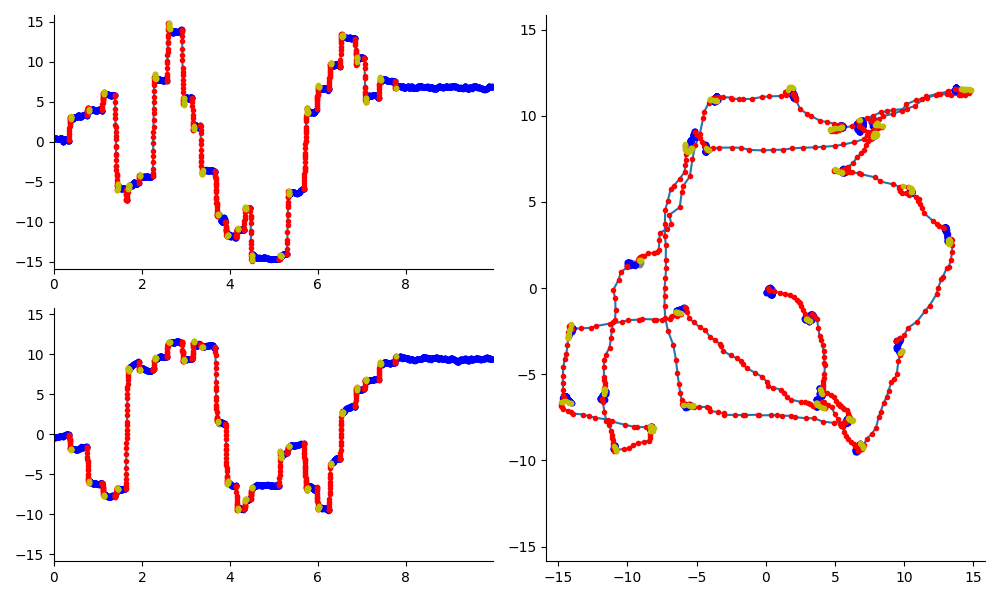
\includegraphics[width=\linewidth]{TH34_img_Europe_labelled_MN}
    \caption{The two graphs on the left show the x and y coordinates of the gaze position in degrees over time in seconds. The graph on the right resembles the gaze position in the x-y-plane. The red dots represent fixations, the blue dots represent saccades and the green dots represent post saccadic oscillations.}
\end{figure}

\section{Conversion script}
In order to allow maximum flexibility for future users of gazeNet a script is provided which converts .csv/.tsv eye tracking data files into the proprietary datatype ETData used by gazeNet. The script works on both Windows and UNIX-like operating systems thanks to pathlib which handles path and file names. Even though slight modification may be necessary, the given script should provide a usefull template for the preparation of similarly formatted gaze recordings.

In this particular case the file to be converted stems from an eye tracker made by Tobii. Each sample of the recording is stored in a separate row. The gaze coordinates are stored in the columns "Gaze point X" and "Gaze point Y" in cartesian form as pixels and can therefore be used as they are. The custom datatype requires information about the geometry of the test setup in order to internally convert the cartesian coordinates to polar coordinates. As of now these parameters are hardcoded in the script. Finally invalid samples are filtered.

\begin{figure}[ht]
    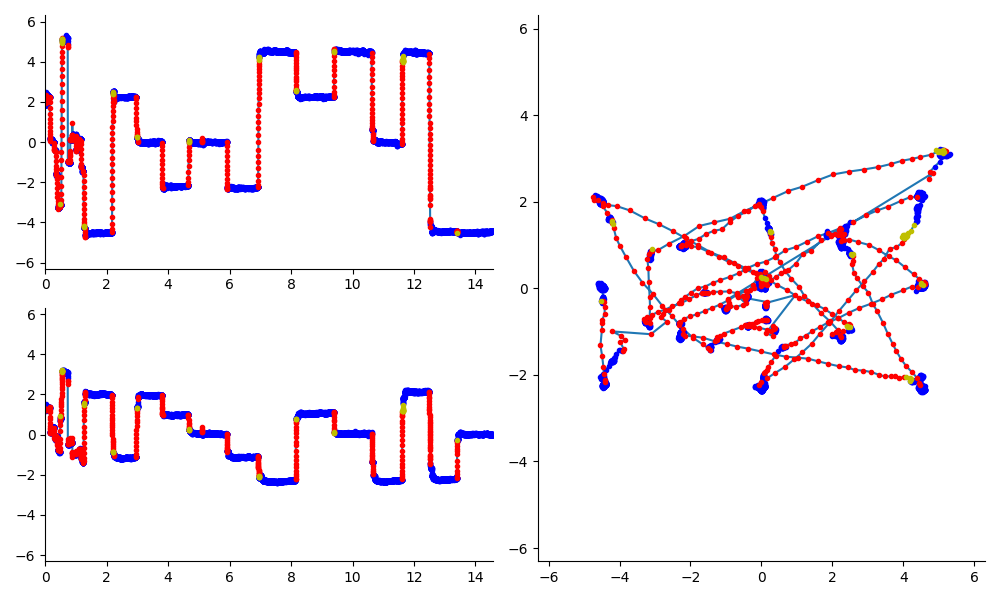
\includegraphics[width=\linewidth]{Kreuze_Random Recording1_short}
    \caption{The two graphs on the left show the x and y coordinates of the gaze position in degrees over time in seconds. The graph on the right resembles the gaze position in the x-y-plane. The red dots represent fixations, the blue dots represent saccades and the green dots represent post saccadic oscillations. It shoud be noted that the first two seconds of the recording contain the calibration points of the eye tracker. The calibration process contains events on which gazeNet is not trained. Therefore the labelling is insignificant.}
\end{figure}


\bibliographystyle{plainnat}
\bibliography{gazeNet.bib}
\end{document}